\documentclass[a4paper,11pt,twoside]{memoir}
\chapterstyle{veelo}

\usepackage{TUINFDA}

\usepackage{url}
\usepackage{hyperref}					% links in pdf
\usepackage{graphicx}            			% Figures
\usepackage{verbatim}            			% Code-Environment
\usepackage[lined,linesnumbered,algochapter]{algorithm2e} % Algorithm-Environment

\usepackage{pgf}					
\usepackage{tikz}					% tikz graphics
\usetikzlibrary{arrows,automata}

\usepackage{ngerman}
\usepackage[ngerman]{babel}
\usepackage{bibgerm,cite}       % Deutsche Bezeichnungen, Automatisches Zusammenfassen von Literaturstellen
\usepackage[ngerman]{varioref}  % Querverweise
% to use the german charset include cp850 for MS-DOS, ansinew for Windows and latin1 for Linux.
% \usepackage[latin1]{inputenc}

\thesistitle{Visualization of program execution in gforth}
\thesissubtitle{Proposal} % optional
\thesisdate{TT.MM.JJJJ}

% all titles and designations have to be gender-related!
\thesisdegree{Bachelor of Science}{Bachelor of Science}
\thesiscurriculum{Software \& Information Engineering}{Software \& Information Engineering} % your study
\thesisverfassung{Verfasserin} % Verfasser
\thesisauthor{Mario Gastegger} % your name
\thesisauthoraddress{Ameisgasse 15/9, 1140 Wien} % your address
\thesismatrikelno{0726289} % your registration number

\thesisbetreins{Ao.Univ.Prof. Dipl.-Ing. Dr.techn. Martin  Ertl}
\thesisbetrzwei{Dr. Vorname Familienname}
\thesisbetrdrei{Dr. Vorname Familienname} % optional

% define page numbering styles
\makepagestyle{numberCorner}
\makeevenfoot{numberCorner}{\thepage}{}{}
\makeoddfoot{numberCorner}{}{}{\thepage}

% define custom macros for specific formats or names
\newcommand{\uml}[1]{\texttt{#1}}
\newcommand{\cd}{\textsf{Class Diagram}}

\begin{document}

\captionnamefont{\bfseries}

%%%%%%%%%%%%%%%%%%%%%%%%%%%%%%%%%%%%%%%%%
%%%   FRONTMATTER    %%%%%%%%%%%%%%%%%%%%
%%%%%%%%%%%%%%%%%%%%%%%%%%%%%%%%%%%%%%%%%
\frontmatter
\pagenumbering{arabic}

%%%%%%%%%%%%%%%%%%%%%%%%%%%%%%%%%%%%%%%%%
%%%   TITLEPAGES    %%%%%%%%%%%%%%%%%%%%%
%%%%%%%%%%%%%%%%%%%%%%%%%%%%%%%%%%%%%%%%%

% the german title page is required as first page
% $Id: titlepage.tex 1752 2010-03-20 11:07:02Z tkren $
%
% TU Wien - Faculty of Informatics
% thesis titlepage
%
% This titlepage is using the geometry package, see
% <http://www.ctan.org/macros/latex/contrib/geometry/geometry.pdf>
%
% For questions and comments send an email to
% Thomas Krennwallner <tkren@kr.tuwien.ac.at>
% or to Petra Brosch <brosch@big.tuwien.ac.at>
%

\selectlanguage{ngerman}

% setup page dimensions for titlepage
\newgeometry{left=2.4cm,right=2.4cm,bottom=2.5cm,top=2cm}

% force baselineskip and parindent
\newlength{\tmpbaselineskip}
\setlength{\tmpbaselineskip}{\baselineskip}
\setlength{\baselineskip}{13.6pt}
\newlength{\tmpparindent}
\setlength{\tmpparindent}{\parindent}
\setlength{\parindent}{17pt}

% first titlepage
\thispagestyle{tuinftitlepage}

%
% Kludge: for each titlepage set \pagenumbering to a different
% style. This is used to fix a problem with hyperref, because there
% are multiple "page 1" and hyperref hates that
%
\pagenumbering{Alph}

\begin{center}
{\ \vspace{3.4cm}}

\begin{minipage}[t][2.8cm][s]{\textwidth}%
\centering
\thesistitlefontHUGE\sffamily\bfseries\tuinfthesistitle\\
\bigskip
{\thesistitlefonthuge\sffamily\bfseries\tuinfthesissubtitle}
\end{minipage}

\vspace{1.3cm}

{\thesistitlefontLARGE\sffamily \tuinfthesistype}

\vspace{6mm}

{\thesistitlefontlarge\sffamily zur Erlangung des akademischen Grades}

\vspace{6mm}

{\thesistitlefontLARGE\sffamily\bfseries \tuinfthesisdegree}

\vspace{6mm}

{\thesistitlefontlarge\sffamily im Rahmen des Studiums}

\vspace{6mm}

{\thesistitlefontLarge\sffamily\bfseries \tuinfthesiscurriculum}

\vspace{6.5mm}

{\thesistitlefontlarge\sffamily eingereicht von}

\vspace{6mm}

{\thesistitlefontLarge\sffamily\bfseries \tuinfthesisauthor}

\vspace{1.5mm}

{\thesistitlefontlarge\sffamily Matrikelnummer \tuinfthesismatrikelno} 

\vspace{1.4cm}

\vspace{0pt}\raggedright\thesistitlefontnormalsize\sffamily
\begin{minipage}[t][1.6cm][t]{\textwidth}%
  %
  an der

  Fakult\"{a}t f\"{u}r Informatik der Technischen Universit\"{a}t Wien
\end{minipage}

\begin{minipage}[t][4cm][t]{\textwidth}%
  \vspace{0pt}\raggedright\thesistitlefontnormalsize\sffamily
  %
  \begin{tabbing}%
	    \hspace{19mm} \= \hspace{66mm} \kill
	    \tuinfthesisbetreuung: \> \tuinfthesisbetreins\\
%	    Mitwirkung: \> \tuinfthesisbetrzwei\\
%	                \> \tuinfthesisbetrdrei
  \end{tabbing}
\end{minipage}

\begin{minipage}[t][1.5cm][t]{\textwidth}%
  \vspace{0pt}\sffamily\thesistitlefontnormalsize
  \begin{tabbing}%
    \hspace{45mm} \= \hspace{63mm} \= \hspace{51mm} \kill
    Wien, \tuinfthesisdate \> {\raggedright\rule{51mm}{0.5pt}} \> {\raggedright\rule{51mm}{0.5pt}} \\
    \> \begin{minipage}[t][0.5cm][t]{51mm}\centering (Unterschrift \tuinfthesisverfassung)\end{minipage}
    \> \begin{minipage}[t][0.5cm][t]{51mm}\centering (Unterschrift \tuinfthesisbetreuung)\end{minipage}
    \end{tabbing}
\end{minipage}

\end{center}

% we want an empty page right after first titlepage
\pagestyle{empty}
\cleardoublepage

% we're done with the titlepages, proceed with default pagenumbering
\pagenumbering{roman}

% restore baselineskip
\setlength{\baselineskip}{\tmpbaselineskip}
\setlength{\parindent}{\tmpparindent}

% back to normal geometry
\restoregeometry

\selectlanguage{english}

%%% Local Variables:
%%% TeX-PDF-mode: t
%%% TeX-debug-bad-boxes: t
%%% TeX-parse-self: t
%%% TeX-auto-save: t
%%% reftex-plug-into-AUCTeX: t
%%% End:


% an english translation may follow
% $Id: titlepage.tex 1752 2010-03-20 11:07:02Z tkren $
%
% TU Wien - Faculty of Informatics
% thesis titlepage
%
% This titlepage is using the geometry package, see
% <http://www.ctan.org/macros/latex/contrib/geometry/geometry.pdf>
%
% For questions and comments send an email to
% Thomas Krennwallner <tkren@kr.tuwien.ac.at>
% or to Petra Brosch <brosch@big.tuwien.ac.at>
%

% setup page dimensions for titlepage
\newgeometry{left=2.4cm,right=2.4cm,bottom=2.5cm,top=2cm}

% force baselineskip and parindent
%\newlength{\tmpbaselineskip}
%\setlength{\tmpbaselineskip}{\baselineskip}
%\setlength{\baselineskip}{13.6pt}
%\newlength{\tmpparindent}
%\setlength{\tmpparindent}{\parindent}
%\setlength{\parindent}{17pt}

% first titlepage
\thispagestyle{tuinftitlepage}

%
% Kludge: for each titlepage set \pagenumbering to a different
% style. This is used to fix a problem with hyperref, because there
% are multiple "page 1" and hyperref hates that
%
\pagenumbering{Roman}

\begin{center}
{\ \vspace{3.4cm}}

\begin{minipage}[t][2.8cm][s]{\textwidth}%
\centering
\thesistitlefontHUGE\sffamily\bfseries\tuinfthesistitle\\
\bigskip
{\thesistitlefonthuge\sffamily\bfseries\tuinfthesissubtitle}
\end{minipage}

\vspace{1.3cm}

{\thesistitlefontLARGE\sffamily \tuinfthesistypeen}

\vspace{6mm}

{\thesistitlefontlarge\sffamily submitted in partial fulfillment of the requirements for the degree of}

\vspace{6mm}

{\thesistitlefontLARGE\sffamily\bfseries \tuinfthesisdegreeen}

\vspace{6mm}

{\thesistitlefontlarge\sffamily in}

\vspace{6mm}

{\thesistitlefontLarge\sffamily\bfseries \tuinfthesiscurriculumen}

\vspace{6.5mm}

{\thesistitlefontlarge\sffamily by}

\vspace{6mm}

{\thesistitlefontLarge\sffamily\bfseries \tuinfthesisauthor}

\vspace{1.5mm}

{\thesistitlefontlarge\sffamily Registration Number \tuinfthesismatrikelno} 

\vspace{1.4cm}

\begin{minipage}[t][1.6cm][t]{\textwidth}%
  \vspace{0pt}\raggedright\thesistitlefontnormalsize\sffamily
  %
  to the Faculty of Informatics 

  at the Vienna University of Technology
\end{minipage}

\vspace{0pt}\raggedright\thesistitlefontnormalsize\sffamily
\begin{minipage}[t][4cm][t]{\textwidth}%
  \begin{tabbing}%
	    \hspace{19mm} \= \hspace{66mm} \kill
	    Advisor: \> \tuinfthesisbetreins\\
%	    Assistance: \> \tuinfthesisbetrzwei\\
%	                \> \tuinfthesisbetrdrei
     \end{tabbing}
\end{minipage}

\begin{minipage}[t][1.5cm][t]{\textwidth}%
  \vspace{0pt}\sffamily\thesistitlefontnormalsize
  \begin{tabbing}%
    \hspace{45mm} \= \hspace{63mm} \= \hspace{51mm} \kill
%    Vienna, \tuinfthesisdate \> {\raggedright\rule{51mm}{0.5pt}} \> {\raggedright\rule{51mm}{0.5pt}} \\
%    \> \begin{minipage}[t][0.5cm][t]{51mm}\centering (Signature of Author)\end{minipage}
%    \> \begin{minipage}[t][0.5cm][t]{51mm}\centering (Signature of Advisor)\end{minipage}
    \end{tabbing}
\end{minipage}

\end{center}

% we want an empty page right after first titlepage
\pagestyle{empty}
\cleardoublepage

% we're done with the titlepages, proceed with default pagenumbering
\pagenumbering{roman}

% restore baselineskip
\setlength{\baselineskip}{\tmpbaselineskip}
\setlength{\parindent}{\tmpparindent}

% back to normal geometry
\restoregeometry


%%% Local Variables:
%%% TeX-PDF-mode: t
%%% TeX-debug-bad-boxes: t
%%% TeX-parse-self: t
%%% TeX-auto-save: t
%%% reftex-plug-into-AUCTeX: t
%%% End:
 % optional

%%%%%%%%%%%%%%%%%%%%%%%%%%%%%%%%%%%%%%%%%
%%%   ERKLAERUNG DER SELBSTAENDIGKEIT   %
%%%%%%%%%%%%%%%%%%%%%%%%%%%%%%%%%%%%%%%%%
%\cleardoublepage
%\selectlanguage{ngerman}
%\chapter*{Erklärung zur Verfassung der Arbeit}

\tuinfthesisauthor\\
\tuinfthesisauthoraddress

\vspace*{1.2cm}

Hiermit erkläre ich, dass ich diese Arbeit selbständig verfasst habe, 
dass ich die verwendeten Quellen und Hilfsmittel vollständig angegeben 
habe und dass ich die Stellen der Arbeit - einschließlich Tabellen, 
Karten und Abbildungen -, die anderen Werken oder dem Internet im 
Wortlaut oder dem Sinn nach entnommen sind, auf jeden Fall unter Angabe 
der Quelle als Entlehnung kenntlich gemacht habe.\\

\vspace*{2cm}
\begin{tabbing}%
    \hspace{58mm} \= \hspace{28mm} \= \hspace{58mm} \kill
    {\raggedright\rule{58mm}{0.5pt}} \> \> {\raggedright\rule{58mm}{0.5pt}} \\
    \begin{minipage}[t][0.5cm][t]{58mm}
	\vspace{0pt}\sffamily\thesistitlefontnormalsize
	\centering (Ort, Datum)
    \end{minipage}
    \> \>
    \begin{minipage}[t][0.5cm][t]{58mm}
	\vspace{0pt}\sffamily\thesistitlefontnormalsize
	\centering (Unterschrift \tuinfthesisverfassung)
    \end{minipage}
\end{tabbing}


%\selectlanguage{english}

%%%%%%%%%%%%%%%%%%%%%%%%%%%%%%%%%%%%%%%%%
%%%   ACKNOWLEDGEMENTS    %%%%%%%%%%%%%%%
%%%%%%%%%%%%%%%%%%%%%%%%%%%%%%%%%%%%%%%%%

% optional acknowledgements may be included in german or in english
%\chapter*{Danksagung}

Hier fügen Sie optional eine Danksagung ein.
 		% optional
%\chapter*{Acknowledgements}

Optional acknowledgements may be inserted here.	% optional

%%%%%%%%%%%%%%%%%%%%%%%%%%%%%%%%%%%%%%%%%
%%%   ABSTARCT    %%%%%%%%%%%%%%%%%%%%%%%
%%%%%%%%%%%%%%%%%%%%%%%%%%%%%%%%%%%%%%%%%

\chapter*{Abstract}

\section{Problem definition}

In software engineering, the most important part is to verify the correctness of a program. The difficulty of this task grows with the size and the complexity of a program. Thus the task of finding faulty code takes a considerable amount of time and the efficiency of finding faulty code a major concern. There a several methods to improve the quality of code.

correctness
faulty code
methods to improve quality
debugging watch and break
in forth/gforth
println method and visualization of program execution
transparent and automated

\section{Expected results}

improvement of awareness of whats happening during execution and efficiency of finding faulty code

\section{Methodology and approach}

\begin{enumerate}
  \item research on program flow visualization
	\item research on forth
  \item research on architecture of gforth
  \item research on ``debugging'' in forth/gforth
  \item research of similar approaches
  \item extracting several technical approaches to accomplish the task(hooks, word-wrapping, level of implementation)
  \item evaluation of the approaches(automation?, performance, feasibility)
  \item prototyping the approaches in order of quality(?)
\end{enumerate}

\section{State of the art}
?

\section{Relation to Software engineering}

\begin{itemize}
	\item software testing(analysis, debugging)
	\item development process(rapid prototyping)
	\item stack-based language forth
\end{itemize}

\section{References}

\begin{itemize}
	\item correctness
	\item software quality
	\item debugging watch and break points
	\item println method
	\item visualization of data manipulation and
	\item program flow
\end{itemize}
\cleardoublepage
%\selectlanguage{ngerman}
%\chapter*{Kurzfassung}

i) Problemstellung, 
ii) erwartetes Resultat, 
iii) methodisches Vorgehen, 
iv) State-of-the art (inkl. mind. vier Literaturreferenzen) sowie 
v) Bezug zum angeführten Studium 
abgefasst werden.
%\selectlanguage{english}

%%%%%%%%%%%%%%%%%%%%%%%%%%%%%%%%%%%%%%%%%
%%%   CONTENTS    %%%%%%%%%%%%%%%%%%%%%%%
%%%%%%%%%%%%%%%%%%%%%%%%%%%%%%%%%%%%%%%%%
% uncomment to set document language to german (results in "Inhaltsverzeichnis", "Kapitel", "Abbildung", etc. instead of "Contents", "Chapter", and "Figure"), otherwise the document's language is english
%\selectlanguage{ngerman}

%\setcounter{tocdepth}{1}

%\cleardoublepage
%\pagestyle{numberCorner}
%\tableofcontents*

%%%%%%%%%%%%%%%%%%%%%%%%%%%%%%%%%%%%%%%%%
%%%   MAINMATTER    %%%%%%%%%%%%%%%%%%%%%
%%%%%%%%%%%%%%%%%%%%%%%%%%%%%%%%%%%%%%%%%

%\mainmatter
%\pagenumbering{arabic}
%\pagestyle{numberCorner}

%%%%%%%%%%%%%%%%%%%%%%%%%%%%%%%%%%%%%%%%%
%\chapter{Introduction}
%\label{ch:intro}
%%%%%%%%%%%%%%%%%%%%%%%%%%%%%%%%%%%%%%%%%

%\chapter{Introduction}

\section*{Motivation}

Software systems underlie continuous changes throughout their whole life cycle.
They evolve from the beginning of development until their release and maintenance phase. Large software systems\footnote{"The term large is, generally, used to describe software whose size in number of lines of code is greater than some arbitrary value. For reasons indicated in [leh79], it is more appropriate to define a large program as one developed by processes involving groups with two or more management levels."\cite{Lehman:2003:SEB:950401.950407}} and most of all, software  classified as type E \cite{Cook:2006:ESS:1115566.1115567}, get more complex over time.\\
If there are more than a few developers/development teams involved or the developers/development teams are spread all over the world, there exists more foreign code than self written code. This makes it necessary to understand foreign code.
Most of all when it comes to making changes, enhancements or fixes, there is a very high level of understanding of the software at hand necessary\cite{Boehm:1976:SE:1311958.1312684}\cite{Singer97anexamination}. Due to \cite{Cornelissen:2009:SSP:1638616.1639301}, "... up to 60\% of the maintenance effort is spent on gaining a sufficient understanding of the program ...". These facts emphasize the need for computer aided methods to improve program understanding.

This thesis addresses the task of improving program comprehension of the concatenative programming language Forth on several levels. The terms "program understanding" and "program comprehension" are considered synonym. Namely the reading of source code, static analysis, dynamic analysis and the assistance of writing readable and easy to understand source code.

Due to the nature of concatenative languages, it is possible to write source code which reads very similar to natural language. There are no hard boundaries to the structure of the source code(custom defined loops and control structures) as in most other languages. Since Forth directly operates only on stacks and memory, the information which is immediately needed to follow the program execution is limited to those structures. In contrast, in object-oriented languages there is also object state, object life cycle and concurrency to keep in mind.

\begin{comment}
\hl{mental model(LaToza et al., 2006) read: ..comment}
\@inproceedings\{Lieberman:1995:BGC:223904.223969,
author = \{Lieberman, Henry and Fry, Christopher\},
title = \{Bridging the Gulf Between Code and Behavior in Programming\},
booktitle = \{Proceedings of the SIGCHI Conference on Human Factors in Computing Systems\},
series = \{CHI '95\},
year = \{1995\},
isbn = \{0-201-84705-1\},
location = \{Denver, Colorado, USA\},
pages = \{480--486\},
numpages = \{7\},
url = \{http://dx.doi.org/10.1145/223904.223969\},
doi = \{10.1145/223904.223969\},
acmid = \{223969\},
publisher = \{ACM Press/Addison-Wesley Publishing Co.\},
address = \{New York, NY, USA\},
\}
\end{comment}


\section*{Problem statement}

There has been done plenty of work on the task of program comprehension in object oriented and procedural languages\cite{Cornelissen:2009:SSP:1638616.1639301}, but nearly none for concatenative languages. \begin{comment} The qualitative exploratory approach of this thesis does not encourage the formulation of specific hypothesis. Therefore the first question, is the applicability of existing methods and their visualization techniques. The second question to be answered, concerns new approaches, which may be exclusive to concatenative languages or Gforth/Forth.\end{comment}

\section*{Aim of the work}

This work aims to give a brief overview on the field of program comprehension and its methods, to show existing aids to program understanding in Gforth/Forth and to study the applicability of some existing analysis and visualization approaches for other paradigms. Furthermore the suggestion of new methods or the modification of existing methods to meet the characteristics of Gforth/Forth.

\section*{Structure of the work}

In Chapter \ref{chap:Methodology}, I will outline the methodological approach of this thesis. In Chapter \ref{chap:StateOfTheArt}, there will be a brief overview on the topic of program comprehension, an overview on the existing tools to improve program understanding in general and on those specific to Gforth/Forth and afterwards I will present a selection of visualization approaches for procedural and object-oriented languages. In Chapter \ref{chap:Results}, I will present some of the previously mentioned approaches for other paradigms applied to a real world Forth program, analyze their applicability and propose modifications to those approaches. Afterwards I will present a prototype implementation of a program trace visualization enhancement to Gforth. Chapter \ref{chap:Summary} concludes the thesis with a summary and topics of further investigation.

\begin{comment}
At first, the available information of a forth program is identified. The next step is to characterize the information and its necessity for program comprehension is investigated. The differences of forth and object oriented languages are summarized and then the applicability of existing analysis and visualization methods is presented. \hl{Since there is no standard implementation of object orientation if forth, this thesis won't take any object orientation implementation into account.}
The last part of this thesis investigates probable enhancements and modifications to existing methods and proposes new approaches.
After the conclusion, the thesis presents further suggestions to support program comprehension and further topics of research in this direction.
\end{comment}

%%%%%%%%%%%%%%%%%%%%%%%%%%%%%%%%%%%%%%%%%
%\chapter{Typographic Design}
%\label{ch:typo}
%%%%%%%%%%%%%%%%%%%%%%%%%%%%%%%%%%%%%%%%%

%
For working with LaTeX you can take advantage of a variety of books and free introductions and tutorials on the internet. A competent contact point for LaTeX beginners is the LaTeX Wikibook, which is available under \url{http://en.wikibooks.org/wiki/LaTeX}. 

The following sections give examples of the most important LaTeX environments and commands.

\section{Tables}

Tables have to be realized with the help of the \textit{table} environment. Tables shall be sequentially numbered for each chapter and described in terms of a short caption (cf. Table~\ref{tab:diplomaseminar}).

\begin{table}[htb]
	\centering
	\begin{tabular}{|l|c|c|}
		\hline \textbf{Name} & \textbf{Date} & \textbf{Title} \\
		\hline
		\hline Mustermann Adam  & 18.5   & T1    \\
		\hline Musterfrau Eva  & 22.6   & T2    \\
		\hline
	\end{tabular}
	\caption{Seminar for Master Students}
	\label{tab:diplomaseminar}
\end{table}


\section{Figures}

Like tables, figures shall be sequentially numbered for each chapter and described in terms of a short caption). You could either produce your drawings directly inside Latex using PSTricks\footnote{\url{http://tug.org/PSTricks}}, Tikz\footnote{\url{http://sourceforge.net/projects/pgf}}, or any set of macros dedicated to your requirements (cf. Figure~\ref{fig:samplefigure_tikz}). Alternatively, you may include figures prepared in external tools (cf. Figure~\ref{fig:samplefigure_pdf}). Note, to ensure high quality printing, all figures must have at least 300 dpi.

\begin{figure}
	\centering
	\begin{tikzpicture}[->, auto, node distance=2.8cm, semithick]
	  \node[initial, state] (1)		 {$S_1$};
	  \node[state] 		(2) [right of=1] {$S_2$};
	
	  \path (1) edge [bend left]  node {0} (2)
		(1) edge [loop above] node {1} (1)
		(2) edge [bend left]  node {0} (1)
		(2) edge [loop above] node {1} (2);
	\end{tikzpicture}
	\caption{Sample figure}
	\label{fig:samplefigure_tikz}
\end{figure}

\begin{figure}[tb]
	\centering
	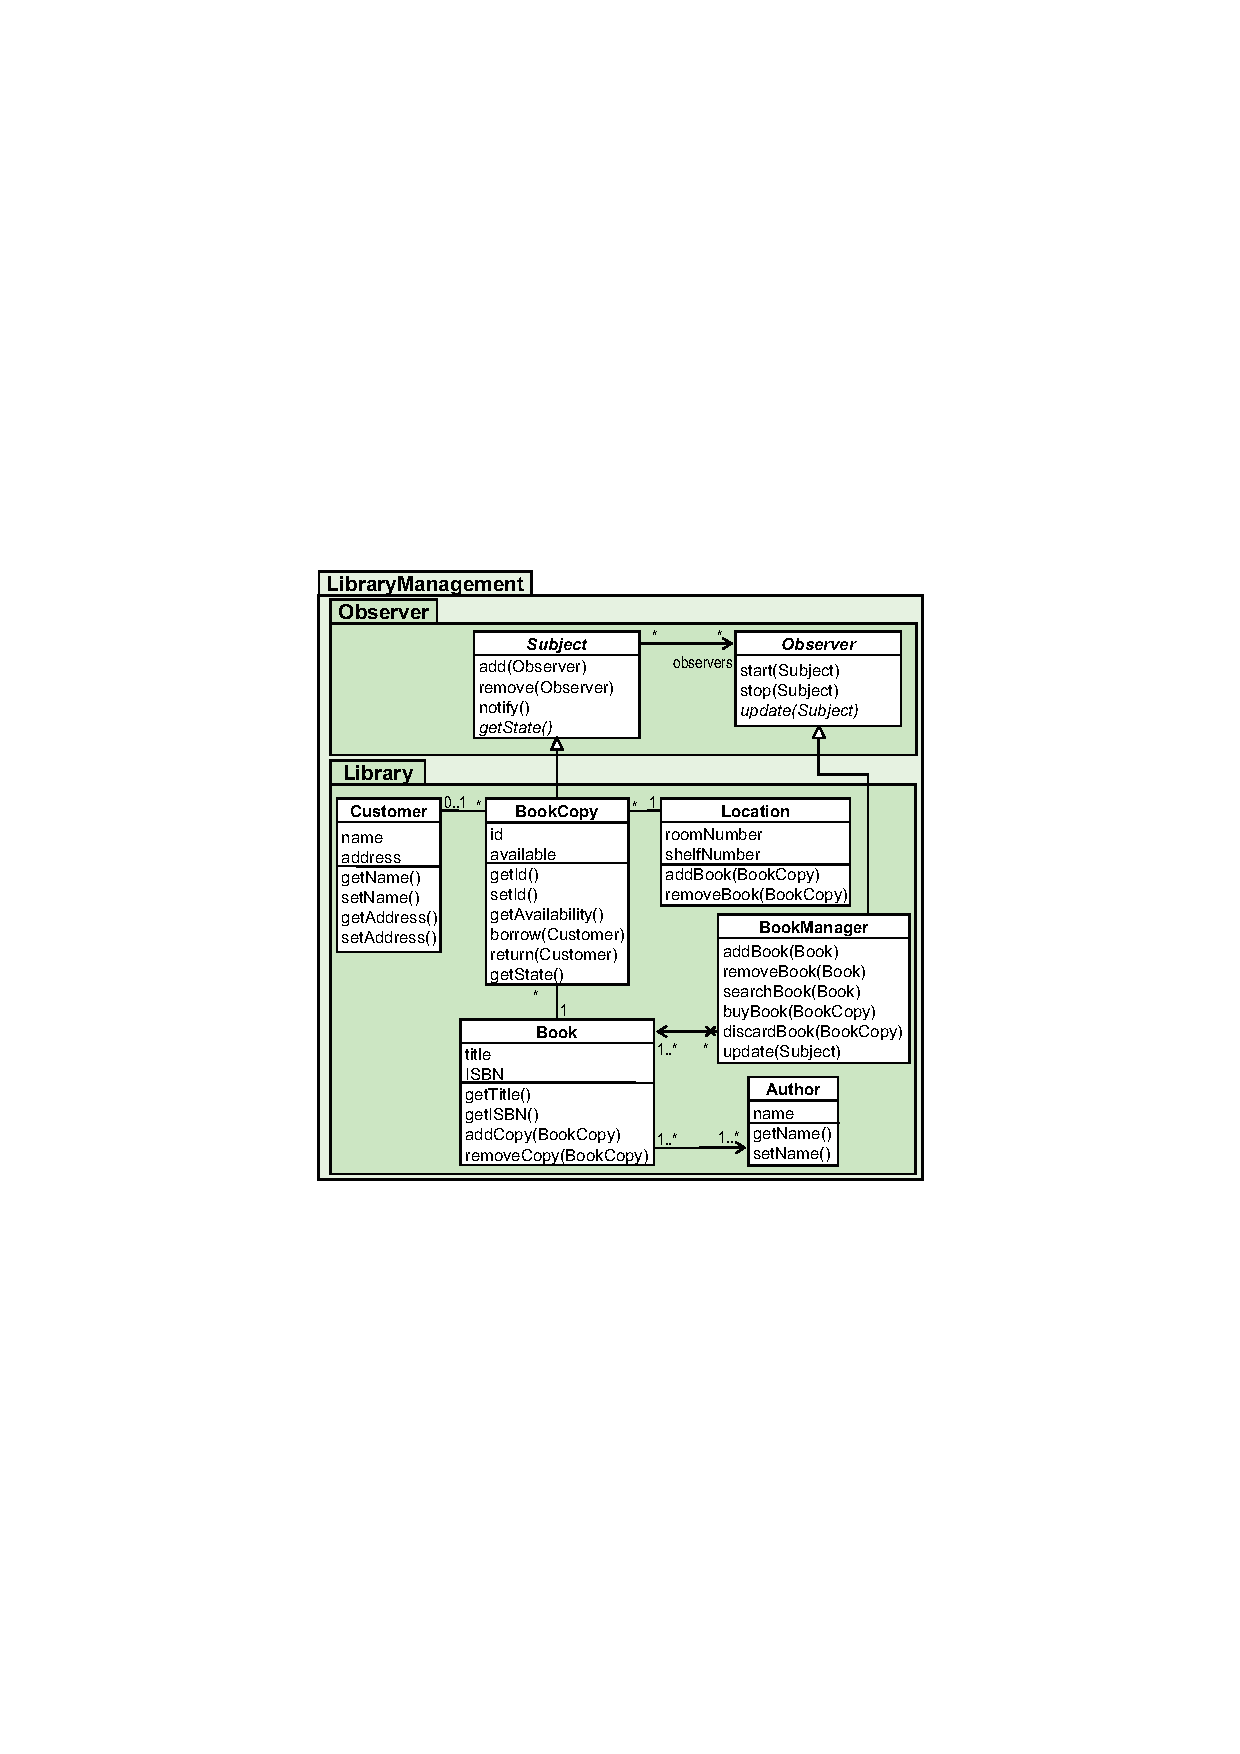
\includegraphics[width=0.7\textwidth]{figures/figure1}
	\caption{Sample figure}
	\label{fig:samplefigure_pdf}
\end{figure}


\section{Fonts}

When introducing important terms for the first time use \emph{emphasize}. For a consistent look and feel of proper names like {\cd} and {\uml{Observer}} pattern you may define macros in the main document \texttt{thesis.tex}.

\section{Code}

For short code fragments use the \textit{verbatim} environment.

\begin{verbatim}
//Start Program
System.out.println("Hello World!");
//End Program
\end{verbatim}

A much better alternative is the \textit{algorithm} environment (cf. Algorithm~\ref{alg:samplealgorithm}). This environment offers special formatting features for loops, operations and comments.

\begin{algorithm}[t]
\SetKwData{Left}{left}
\SetKwData{This}{this}
\SetKwData{Up}{up}
\SetKwFunction{Union}{Union}
\SetKwFunction{FindCompress}{FindCompress}
\SetKwInOut{Input}{input}
\SetKwInOut{Output}{output}

\Input{A bitmap $Im$ of size $w\times l$}
\Output{A partition of the bitmap}

\BlankLine

\emph{special treatment of the first line}\;
\For{$i\leftarrow 2$ \KwTo $l$}{
\emph{special treatment of the first element of line $i$}\;
\For{$j\leftarrow 2$ \KwTo $w$}{\label{forins}
\Left$\leftarrow$ \FindCompress{$Im[i,j-1]$}\;
\Up$\leftarrow$ \FindCompress{$Im[i-1,]$}\;
\This$\leftarrow$ \FindCompress{$Im[i,j]$}\;
\If(\tcp*[r]{O(\Left,\This)==1}){\Left compatible with \This}{\label{lt}
\lIf{\Left $<$ \This}{\Union{\Left,\This}}\;
\lElse{\Union{\This,\Left}\;}
}
\If(\tcp*[r]{O(\Up,\This)==1}){\Up compatible with \This}{\label{ut}
\lIf{\Up $<$ \This}{\Union{\Up,\This}}\;
\tcp{\This is put under \Up to keep tree as flat as possible}\label{cmt}
\lElse{\Union{\This,\Up}}\tcp*[r]{\This linked to \Up}\label{lelse}
}
}
\lForEach{element $e$ of the line $i$}{\FindCompress{p}}
}
\caption{Sample algorithm}\label{alg:samplealgorithm}
\end{algorithm}



%%%%%%%%%%%%%%%%%%%%%%%%%%%%%%%%%%%%%%%%%
%\chapter{Bibliographic Issues}
%\label{ch:bibliographic}
%%%%%%%%%%%%%%%%%%%%%%%%%%%%%%%%%%%%%%%%%

%\section{Literature Search}

Information on online libraries and literature search, e.g., interesting magazines, journals, conferences, and organizations may be found at \url{http://www.big.tuwien.ac.at/teaching/info.html}.

\section{BibTeX}

BibTeX should be used for referencing.

The LaTeX source document of this pdf document provides you with different samples for references to journals~\cite{jour:B2BServices}, conference papers~\cite{proc:TheWebMLApproach}, books~\cite{book:umlatwork}, book chapters~\cite{incoll:ErhardKonrad1992}, electronic standards~\cite{man:BPEL}, dissertations~\cite{phdthesis:manuelWimmer}, masters' theses~\cite{mast:AUMLProfile}, and web sites~\cite{misc:BIGWebsite}. The respective BibTeX entries may be found in the file \texttt{references.bib}. For administration of the BibTeX references we recommend \url{http://www.citeulike.org} or JabRef for offline administration, respectively.


%%%%%%%%%%%%%%%%%%%%%%%%%%%%%%%%%%%%%%%%%
%%% BACKMATTER %%%%%%%%%%%%%%%%%%%%%%%%%%
%%%%%%%%%%%%%%%%%%%%%%%%%%%%%%%%%%%%%%%%%

%\appendix

%\bibliographystyle{plain}
%\bibliography{references}

\end{document}
